%{\let\clearpage\relax \chapter{Existing Work}}
\chapter{Existing Work}

% TODO: Change, no longer doing actual analysis
%While to our knowledge no work exists that statistically analyses conversations on a large scale, the methods of analysis that we employ are common and well established. The first part of our analysis, in which we analyse a conversation as a string of many small \glspl{da} rests on \gls{da} classification and is addressed in Sec. \ref{ssec: da classification}. The second part of our analysis, which is concerned with analysing conversations as a trajectory through a semantic topic-space, uses topic modelling. Previous topic modelling work is explored in Sec. \ref{sec: topic analysis} -- \ref{ssec: topic labelling}.

In this chapter we introduce previous work within the well-established and active field of \textbf{\gls{da} classification} and within the less active area of \textbf{topic extraction}. We later build upon these methods to build state of the art algorithms within both areas. 
Methods for \gls{da} classification, in which sentences are automatically matched to their \glspl{da} (e.g. "Hello!" $\rightarrow$ greeting, see Sec. \ref{ssec: DAs}), are introduced in Sec. \ref{ssec: da classification}.

Existing methods for topic modelling, which finds out \textit{which} topics are featured within a conversation and \textit{when}, are introduced in Sec. \ref{sec: topic analysis} -- \ref{ssec: topic labelling}.

\section{Dialogue Act Classification \label{ssec: da classification}}
    Dialogue acts (see Sec. \ref{ssec: DAs}) are often applied within the context of adjacency pairs (see \ref{ssec: adjacency pairs}). They have been used to analyse performance appraisal interviews\cite{ap_interview}, predict psychological disorders such as depression or social anxiety\cite{ap_psychological} or analyse politician's speech patterns\cite{ap_trump}.
    A lot of these are based on manually annotated transcriptions or are purely qualitative in nature. To automate DA annotation would make it significantly easier for researchers to process large data sets and quantify their findings. A model for classifying DAs could be written as 
    \begin{equation}
        \hat{f}_{da}: u_i \rightarrow l_i,
    \end{equation}
    where an utterance $u_i$ is mapped to a DA label $l_i$. Better models don't just map one utterance to one label, but consider the whole sequence of utterances $\mathcal{U}$ i.e.
    \begin{equation}
        \hat{f}_{da}: \mathcal{U} \rightarrow \mathcal{L}, \hspace{3em} u_i \in \mathcal{U}, \hspace{0.5em} l_i \in \mathcal{L} \hspace{0.5em} \forall \hspace{0.5em} i.
    \end{equation}
    
    DA classification is an active area of research and different neural network architectures are proposed to improve model performance. State of the art models for DA classification are summarised in \cite{DAgithub}. The comparison is shown in table \ref{table: da models}.
    
    \begin{table}[h]
    \centering
    \begin{tabular}{|l|l|l|}
    \hline
    \textbf{Model}                   & \textbf{Accuracy} & \textbf{Paper / Source}      \\ \hline
    SGNN                             & 83.1              & Ravi et al., 2018 \cite{ravi2018self}   \\ \hline
    CASA                             & 82.9              & Raheja et al., 2019\cite{raheja2019dialogue} \\ \hline
    DAH-CRF                          & 82.3              & Li et al., 2019 \cite{li2018dual}     \\ \hline
    ALDMN                            & 81.5              & Wan et al., 2018 \cite{wan2018improved}    \\ \hline
    CRF-ASN                          & 81.3              & Chen et al., 2018 \cite{chen2018dialogue}   \\ \hline
    Bi-LSTM-CRF                      & 79.2              & Kumar et al., 2017 \cite{kumar2017dialogue}  \\ \hline
    RNN with 3 utterances in context & 77.34             & Bothe et al., 2018 \cite{bothe2018context}  \\ \hline
    \end{tabular}
    \caption{State of the art models and their accuracies. Trained and evaluated on the SwDa corpus. There was only 84\% agreement among human annotators of the SwDa corpus, so the best models are almost as accurate as humans.\cite{swda}.}
    \label{table: da models}
    \end{table}
    
    \subsection{Bi-LSTM-CRF \label{sssec: kumar model}}
    For our work, we select the Bi-LSTM-CRF model\cite{kumar2017dialogue}, because of high model accuracy and because the authors released their source code. It combines a bidirectional recurrent network using LSTM neurons (see Sec. \ref{ssec: RNNs}) with a conditional random field (CRF) layer and word embeddings. Since we made changes to the model and re-implemented it, a more thorough explanation of the Bi-LSTM-CRF model along with a plot of the model (Fig. \ref{fig:kumar_model} can be found in the method section \ref{ssec: bi-lstm-crf} %TODO: Make CRF section

\section{Topic Extraction \label{sec: topic analysis}}

While \gls{da} classification is extensively and actively researched specifically within the context of conversations, topic extraction is not. Many techniques that work well in well-structured, regular text documents (such as newspaper articles or scientific papers) struggle within the context of conversations. These techniques, and the sparse attempts to apply them to conversations, are summarised in this section.

The usual approach to analysing topics in text is
\begin{enumerate}
    \item Segment the text into its different topics, i.e. determine where a topic changes (Sec. \ref{ssec: topic segmentation}).
    \item Label every segment with a topic, i.e. determine what a given segment is about (Sec. \ref{ssec: topic labelling}).
\end{enumerate}
Some methods, such as Purver et al.\cite{purver2006unsupervised}, do both at the same time.

Topic Extraction is used in a wide number of applications, for example in companies' live-chats, that automatically classify customer issues and send them to the most applicable support teams, or in content-sharing sites such as YouTube, that automatically generate tags for posts and videos to improve content recommendation\cite{queryClassification}. 
\section{Topic Segmentation \label{ssec: topic segmentation}}
Topic segmentation is a procedure that divides a text into sections, where each section significantly differs semantically from the previous. 
Consider the beginning of a conversation between podcast-host Joe Rogan and entrepreneur Elon Musk:\\

\BrText{$t_1$}{
    \begin{dialogue}
        
        \speak{Joe Rogan} Welcome back.
        
        \speak{Elon Musk}
        Here we go again.
        
        \speak{Joe Rogan}
        Great to see you and congratulations.
        \speak{Elon Musk}
        Thank you.
    \end{dialogue}
}

\vspace{1em} 
\hspace{2.5em} \myrulefill{20em}{\textsc{Topic Divider}}
\vspace{1em}
        
\BrText{$t_2$}{ 
    \begin{dialogue}
         
        
        \speak{Joe Rogan}
        You will never forget what is going on in the world when you think about when your child is born. You will know for the rest of this child’s life, you were born during a weird time.
        
        \speak{Elon Musk} [...]
    \end{dialogue}
}
\vspace{-0.3em}\\

\noindent A good topic segmentation algorithm splits this section of conversation at the indicated divider, where the topic changes from greetings to the birth of Elon Musk's child.


There are many approaches to topic segmentation that we explore. They are introduced in this section.

    %\subsection{Lexical Chain Segmentation} 
    %Lexical chain-based methods (such as LCSeg\cite{galley2003discourse}) try to identify semantically related sequences of words (lexical chains) based on term repetitions and then weights them according to frequency (chains containing more repeated terms receive a higher score) and chain length (shorter chains are more likely to be part of the same cohesive structure).\cite{galley2003discourse} \cite{hsueh2006automatic}. LCSeg is public and open for use.
    
    \subsection{Graph-based Segmentation} 
    Graph-based methods represent conversations as a fully connected weighted graph: nodes represent \glspl{utterance} $u_i$ and the weight of edges between nodes $u_i, u_j$ represent some measure of similarity $\eta_{ij}$ between $u_i, u_j$ (such as the cosine similarity between the two \gls{utterance} \glspl{embedding}, as is layed out in Sec. \ref{ssec: utterance embeddings}). Once the conversation is represented as a graph, a threshold weight $\eta_{\text{min}}$ between edges can be set, below which edges are removed. The remaining clusters of sentences defined by remaining edges give the segmentation of the conversation.\cite{malioutov2006minimum} A minimal example is shown in Fig. \ref{fig: graph seg}.
    
    \begin{figure}[ht]
    \centering
    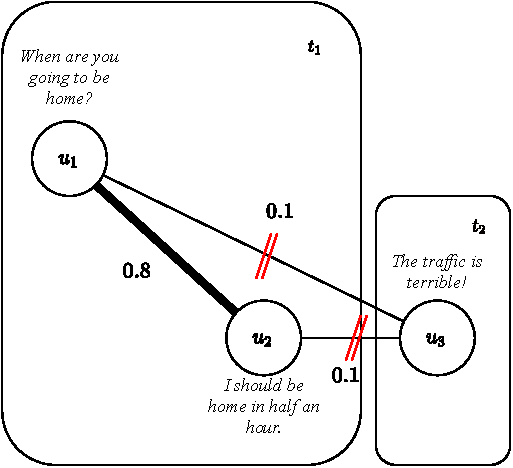
\includegraphics[width=0.7\textwidth]{graphSeg.pdf}
    \caption{Semantically different \glspl{utterance} have their connecting edge cut. The remaining clusters represent topics.\label{fig: graph seg}}
    \end{figure}
     
    \subsection{Bayesian Models}
    Some segmentation methods\cite{eisenstein2008bayesian, purver2006unsupervised, nguyen2012sits} combine segmentation with labelling using \gls{lda}. This is explored further in Sec. \ref{ssec: LDA}.
\section{Topic Labelling \label{ssec: topic labelling}}

Once a document has been segmented into semantically similar regions, for most tasks, they need to be labelled. There are two approaches to this:

\begin{enumerate}
    \item Supervised text classification, where every text is labelled with one (or multiple) topic-labels from a \textbf{predetermined set}\cite{surverTextClassification}. For example, one could label a newspaper article with a label from the set \{politics, sports, weather, finance \dots\}.
    \item Unsupervised topic modelling, where topic-labels are sets of words \textbf{contained within the document itself} and need to first be extracted.
\end{enumerate}

Text classification is often more accurate, but requires the user to impose a finite set of topics that a section can belong to. We explicitly want to avoid imposing a finite set of topics onto the conversations we analyse, so our analysis falls into the area of topic modelling. Common methods are explored here.


\subsection{Latent Dirichlet Allocation \label{ssec: LDA}}
    Latent Dirichlet allocation (LDA)\cite{blei2003latent} is the most common method for topic modelling. It was initially designed to model the topics of \textit{documents} within a \textit{corpus}, such as newspaper articles within an archive of newspapers. LDA is then capable of identifying words belonging to the same topic. The number of topics $k$ is a parameter of LDA and is set by the user.
    Within the context of conversations, the \textit{documents} are the conversation transcripts and the \textit{corpus} is the set of all transcripts.
    
    LDA is a \textit{generative model}, which makes the following assumptions about how a document is generated: There are $k$ topics that any word can be about e.g. $k=3$, where the topics are music, cooking and politics. Each of these topics is made up by the following words with an associated probability of appearing:
    \begin{align*}
        \textbf{Music:  }& \text{[(rock, 1\%), (pop, 0.8\%), (Mozart, 0.4\%), (mp3, 0.2\%), (Beatles, 0.2\%), \dots]}\\
        \textbf{Cooking:    }& \text{[(steak, 2.0\%), (dinner, 1.2\%), (knife, 1.0\%), (delicious, 0.6\%), \dots]}\\
        \textbf{Politics:   }& \text{[(Senate, 2.2\%), (MP, 1.8\%), (Trump, 0.9\%), (debating, 0.3\%), \dots]}.
    \end{align*} 
     
    Now, a document (such as a podcast transcript) is generated in the following way:
     
    \begin{enumerate}
        \item Choose a length of the document e.g. 1000 words.
        \item Choose a set of topics, as well as their probabilities of appearance within the document, e.g. \{(music, 80\%), (cooking, 20\%)\}
    \end{enumerate}
    
    For each word:
    \begin{enumerate}[leftmargin=6em]
    \setcounter{enumi}{2}
        \item A topic is randomly selected: with 80\% probability the topic is music with 20\% probability it is cooking.
        \item From within that topic (say music), a random word is selected with its given probability, e.g. 1\% of the time, the word ``rock" is chosen.
    \end{enumerate}
    
    The real model works \textbf{backwards} from these assumptions to compute the most likely parameters given the observed corpus.
    Mathemathically, LDA determines the parameters that are most likely to have generated the corpus by computing the probability of obtaining a given corpus $D$:
    
    \begin{equation}
        p(D \mid \alpha, \beta)=\prod_{d=1}^{M} \int p\left(T_{d} \mid \alpha\right)\left(\prod_{n=1}^{N_{d}} \sum_{z_{d n}} p\left(z_{d n} \mid T_{d}\right) p\left(w_{d n} \mid z_{d n}, \beta\right)\right) d T_{d},
    \end{equation}
    
    where $\alpha$ and $\beta$ are the parameters we would like to determine,
    the first product is over all $M$ documents $d$,
    the integral is over all possible sets (and probabilities) of topics $T_d$ included in $d$, 
    the second product is over all $N_d$ words that document $d$ contains, where $w_n$ is the $n^{th}$ word.
    The sum is over all topics $z_{dn}$, within $T_d$.
    The term after the sum can be recognised as the probability of drawing the word $w_{dn}$ after drawing the topic $z_{dn}$, which originates in the generative nature of the model.
    The term in the brackets is then the probability of drawing the entire document given that the random variable representing the set of topics is drawn to be $T_d$.
    
    Here, the parameter $\beta$ is a matrix containing the probabilities of every word to appear within every topic, and the parameter $\alpha$ is used as a parameter for drawing the set of topics $T_d$ from a Dirichlet distribution:
    
    \begin{equation}
        p(T \mid \alpha)=\frac{\Gamma\left(\sum_{i=1}^{k} \alpha_{i}\right)}{\prod_{i=1}^{k} \Gamma\left(\alpha_{i}\right)} T_{1}^{\alpha_{1}-1} \cdots T_{k}^{\alpha_{k}-1},
    \end{equation}
    where $k$ is the number of topics and the $d$ in the subscript of $T_d$ is replaced by the topic label for clarity. $\alpha$ is a $k$-dimensional vector with elements $> 0$ and $\Gamma(x)$ is the Gamma function.
    
    Once the LDA model is trained (i.e. a steady state of topic assignments exists), every word can be assigned a topic. By simple majority of topics within a segment, the segment can be labelled.
    
    \subsubsection{Limitations}
    LDA works very well when applied to similarly structured, similar length documents such as news articles\cite{blei2003latent, newman2006probabilistic} or scientific papers\cite{griffiths2004finding, wang2011collaborative}, but is known to struggle with documents that are too short, such as tweets and queries, or documents that contain many topics, such as books\cite{tang2014understanding}. Other weaknesses that are relevant to conversations include:
    
    \begin{itemize}
        \item The number $k$ of topics is fixed and must be subjectively imposed.
        \item Topics are uncorrelated as the Dirichlet topic distribution cannot capture correlations.
        \item Bag of word model: temporal evolution of topics can not be modelled as only word \textbf{counts} across the whole document are considered.
    \end{itemize}
    
    \subsubsection{LDA for Conversations \label{sssec: lda for conversations}}
    Conversations are irregular. They can contain many topics or are focused on just one, every topics can be described by many fitting words or by very few and conversation lengths vary significantly. In conjunction with mis-transcribed words that dilute topics, these issues mean that the generative LDA model, that assumes all documents are generated by the same ``recipe" does not perform well in this medium\cite{purver2006unsupervised, tang2014understanding}. A modified generative approach based on LDA is proposed independently by both Purver et al.\cite{purver2006unsupervised} and Eisenstein et al.\cite{eisenstein2008bayesian}, both of which specifically apply it to multi-party spoken discourse from recorded business meetings aggregated in the ICSI-MRDA corpus\cite{shriberg2004icsi}.
    
    \subsection{Keyphrase Extraction \label{ssec: keyphrase extraction}}
    Another, perhaps simpler, approach is to extract keyphrases (single or multi-word expressions that represent the main topics of a text) from the segmented sections in a process known as keyphrase extraction\cite{hasan2014automatic}. The extracted keyphrases (such as all nouns) represent the topic of the section.
    
    There are many keyphrase extraction methods, the one we evaluate is a graph-based model called TopicRank\cite{bougouin-etal-2013-topicrank}. Here, keyphrase candidates are extracted as noun phrases (phrases that grammatically act like nouns), such as:
    
    \begin{itemize}
        \item \textbf{The spotted puppy} is up for adoption.
        \item \textbf{The car wash} was out of order.
        \item She kindly offered water to \textbf{the gardener working in the hot sun.}
    \end{itemize}
    
    These phrases are identified using part of speech (POS) tagging.
        \subsubsection{Part of Speech Tagging \label{sssec: POS tagging}}
        
        Part of speech (POS) taggers are models 
        \begin{equation}
          \hat{f}_{\text{pos}}: \mathcal{S} \rightarrow \mathcal{P},
        \end{equation} 
        that label sequences of words $\mathcal{S}$(such as the words in a sentence) with their appropriate grammatical function $\mathcal{P}$, known as their part of speech tag. For example:
        
        \begin{equation*}
        \text{[The, house, is, green] $\rightarrow$ [article, noun, verb, adjective]}.
        \end{equation*}
        This tagging problem is approached almost exactly like the dialogue act tagging from Sec. \ref{ssec: da classification}.
        
        \subsubsection{Named Entity Recognition \label{sssec: NER}}
        Named entity recognition (NER) models
        \begin{equation}
          \hat{f}_{\text{ner}}: \mathcal{S} \rightarrow \mathcal{N},
        \end{equation} 
        extract words $\mathcal{N}$ in sequences of words $\mathcal{S}$ that describe a named entity such as a person, company or date and label them accordingly. For example:
        
        \begin{align*}
        \text{[Bill Gates, founded, Microsoft, in, 1975]} \rightarrow [& (\text{Bill Gates, person}), \\
                                                                       & (\text{Microsoft, company}), \\
                                                                       & (\text{1975, year})].
        \end{align*}
        This tagging problem is also approached almost exactly like the dialogue act tagging from Sec. \ref{ssec: da classification}.
        
        \subsubsection{Topic Clustering}
        
        Keyphrase-candidates are grouped into ``topics" if they share at least 25\% of words, excluding stop-words (which are words that don't add meaning, such as ``the").\cite{bougouin-etal-2013-topicrank}
        
        \subsubsection{Graph-Based Ranking}
        After keyphrase-candidates $c_i$ are extracted, the whole document is represented by a complete graph $G = (V, E)$, in which the vertices $V$ are topics $t_i$ and edges $E$ between two topics $t_i$ and $t_j$ are weighted according to the strength of their semantic relation. Here, two topics have a strong semantic relation if they appear close to each other in the document. Formally, the weights are defined to be
            \begin{align}
                w_{i, j} &=\sum_{c_{i} \in t_{i}} \sum_{c_{j} \in t_{j}} \operatorname{dist}\left(c_{i}, c_{j}\right) \\
                \operatorname{dist}\left(c_{i}, c_{j}\right) &=\sum_{p_{i} \in \operatorname{pos}\left(c_{i}\right)} \sum_{p_{j} \in \operatorname{pos}\left(c_{j}\right)} \frac{1}{\left|p_{i}-p_{j}\right|},
            \end{align}
        where pos$(c_i)$ represents all the offset positions (i.e. indices) of the candidate keyphrase $c_i$ within the document.
        
        The topics are then ranked according to the concept of ``voting": high-scoring topics contribute more to the score $S(t_j)$ of their connected topics $t_j$:
        
        \begin{equation}
            S\left(t_{i}\right)=(1-\lambda)+\lambda \times \sum_{t_{j} \in V_{i}} \frac{w_{j, i} \times S\left(t_{j}\right)}{\sum_{t_{k} \in V_{j}} w_{j, k}},
        \end{equation}
        where $V_i$ are the topics voting for $t_i$ and $\lambda$ is a damping factor.
        
        \subsubsection{Extracting the Topic-phrase}
        For each topic, only the most representative keyphrase candidate is selected as the phrase representing the topic. This topic-phrase is extracted for every topic $t_i$ by one of three different methods:
        \begin{enumerate}
            \item The keyphrase candidate that appears first in the document is the topic-phrase.
            \item The most frequent keyphrase candidate is the topic-phrase.
            \item The centroid of all candidates within $t_i$, which is defined to be the candidate most similar to all other candidates is the topic-phrase.\cite{bougouin-etal-2013-topicrank}
        \end{enumerate}
    
    The final topic labels are then defined by the topic-phrases above some minimum rank contained within the segment. This threshold allows the user to define a sensitivity for what constitutes a topic and what does not.
    
        \subsubsection{Limitations}
        Similarly to LDA, TopicRank performs very well when applied well-structured data such as journal papers, but is not evaluated for conversations.\cite{bougouin-etal-2013-topicrank}
     
    \section{Keyphrase Extraction \label{ssec: keyphrase extraction}}
    One labelling approach is the extraction of \glspl{keyphrase} (single or multi-word expressions that represent the main topics of a text) from the segmented sections\cite{hasan2014automatic}. The extracted \glspl{keyphrase} (such as all nouns) represent the topic of the section.
    
    There are many \gls{keyphrase} extraction methods, the one we evaluate is a graph-based model called TopicRank\cite{bougouin-etal-2013-topicrank}. Here, \gls{keyphrase} candidates are extracted as noun phrases (phrases that grammatically act like nouns), such as:
    
    \begin{itemize}
        \item \textbf{The spotted puppy} is up for adoption.
        \item \textbf{The car wash} was out of order.
        \item She kindly offered water to \textbf{the gardener working in the hot sun.}
    \end{itemize}
    
    These phrases are identified using part of speech tagging.
        \subsection{Part of Speech Tagging \label{sssec: POS tagging}}
        
        \Gls{pos} taggers are models 
        \begin{equation}
          \hat{f}_{\text{pos}}: \mathcal{S} \rightarrow \mathcal{P},
        \end{equation} 
        that label sequences of words $\mathcal{S}$(such as the words in a sentence) with their appropriate grammatical function $\mathcal{P}$, known as their part of speech tag. For example:
        
        \begin{equation*}
        \text{[The, house, is, green] $\rightarrow$ [article, noun, verb, adjective]}.
        \end{equation*}
        This tagging problem is approached almost exactly like the \gls{da} tagging from Sec. \ref{ssec: da classification}.
        
        
        \subsection{Topic Clustering}
        
        \Gls{keyphrase}-candidates are grouped into ``topics" if they share at least 25\% of words, excluding stop-words (which are words that don't add meaning, such as ``the").\cite{bougouin-etal-2013-topicrank}
        
        \subsection{Graph-Based Ranking}
        After \gls{keyphrase}-candidates $c_i$ are extracted, the whole document is represented by a complete graph $G = (V, E)$, in which the vertices $V$ are topics $t_i$ and edges $E$ between two topics $t_i$ and $t_j$ are weighted according to the strength of their semantic relation. Here, two topics have a strong semantic relation if they appear close to each other in the document. Formally, the weights are defined to be
            \begin{align}
                w_{i, j} &=\sum_{c_{i} \in t_{i}} \sum_{c_{j} \in t_{j}} \operatorname{dist}\left(c_{i}, c_{j}\right) \\
                \operatorname{dist}\left(c_{i}, c_{j}\right) &=\sum_{p_{i} \in \operatorname{pos}\left(c_{i}\right)} \sum_{p_{j} \in \operatorname{pos}\left(c_{j}\right)} \frac{1}{\left|p_{i}-p_{j}\right|},
            \end{align}
        where pos$(c_i)$ represents all the offset positions (i.e. indices) of the candidate \gls{keyphrase} $c_i$ within the document.
        
        The topics are then ranked according to the concept of ``voting": high-scoring topics contribute more to the score $S(t_j)$ of their connected topics $t_j$:
        
        \begin{equation}
            S\left(t_{i}\right)=(1-\lambda)+\lambda \sum_{t_{j} \in V_{i}} \frac{w_{j, i} S\left(t_{j}\right)}{\sum_{t_{k} \in V_{j}} w_{j, k}},
        \end{equation}
        where $V_i$ are the topics voting for $t_i$ and $\lambda$ is a damping factor.
        
        \subsection{Extracting the Topic-phrase}
        For each topic, only the most representative \gls{keyphrase} candidate is selected as the phrase representing the topic. This topic-phrase is extracted for every topic $t_i$ by one of three different methods:
        \begin{enumerate}
            \item The \gls{keyphrase} candidate that appears first in the document is the topic-phrase.
            \item The most frequent \gls{keyphrase} candidate is the topic-phrase.
            \item The centroid of all candidates within $t_i$, which is defined to be the candidate most similar to all other candidates is the topic-phrase.\cite{bougouin-etal-2013-topicrank}
        \end{enumerate}
    
    The final topic labels are then defined by the topic-phrases above some minimum rank contained within the segment. This threshold allows the user to define a sensitivity for what constitutes a topic and what does not.
    
        %\subsection{Limitations}
        %Similarly to \gls{lda}, TopicRank performs very well when applied to well-structured data such as journal papers, but is not evaluated for conversations.\cite{bougouin-etal-2013-topicrank}
\section{Latent Dirichlet Allocation \label{ssec: LDA}}
    \Gls{lda}\cite{blei2003latent} is the most common method for topic modelling. It was initially designed to model the topics of \textit{documents} within a \textit{corpus}, such as newspaper articles within an archive of newspapers. \gls{lda} is then capable of identifying words belonging to the same topic. The number of topics $k$ is a parameter of \gls{lda} and is set by the user.
    Within the context of conversations, the \textit{documents} are the conversation transcripts and the \textit{corpus} is the set of all transcripts.
    
    \gls{lda} is a \textit{generative model}, which makes the following assumptions about how a document is generated: There are $k$ topics that any word can be about e.g. $k=3$, where the topics are music, cooking and politics. Each of these topics is made up by the following words with an associated probability of appearing:
    \begin{align*}
        \textbf{Music:  }& \text{[(rock, 1\%), (pop, 0.8\%), (Mozart, 0.4\%), (mp3, 0.2\%), (Beatles, 0.2\%), \dots]}\\
        \textbf{Cooking:    }& \text{[(steak, 2.0\%), (dinner, 1.2\%), (knife, 1.0\%), (delicious, 0.6\%), \dots]}\\
        \textbf{Politics:   }& \text{[(Senate, 2.2\%), (MP, 1.8\%), (Trump, 0.9\%), (debating, 0.3\%), \dots]}.
    \end{align*} 
     
    Now, a document (such as a podcast transcript) is generated in the following way:
     
    \begin{enumerate}
        \item Choose a length of the document e.g. 1000 words.
        \item Choose a set of topics, as well as their probabilities of appearance within the document, e.g. \{(music, 80\%), (cooking, 20\%)\}
    \end{enumerate}
    
    For each word:
    \begin{enumerate}[leftmargin=6em]
    \setcounter{enumi}{2}
        \item A topic is randomly selected: with 80\% probability the topic is music with 20\% probability it is cooking.
        \item From within that topic (say music), a random word is selected with its given probability, e.g. 1\% of the time, the word ``rock" is chosen.
    \end{enumerate}
    
    The real model works \textbf{backwards} from these assumptions to compute the most likely parameters given the observed corpus.
    Mathematically, \gls{lda} determines the parameters that are most likely to have generated the corpus by computing the probability of obtaining a given corpus $D$:
    
    \begin{equation}
        p(D \mid \alpha, \beta)=\prod_{d=1}^{M} \int p\left(T_{d} \mid \alpha\right)\left(\prod_{n=1}^{N_{d}} \sum_{z_{d n}} p\left(z_{d n} \mid T_{d}\right) p\left(w_{d n} \mid z_{d n}, \beta\right)\right) d T_{d},
    \end{equation}
    
    where $\alpha$ and $\beta$ are the parameters we would like to determine,
    the first product is over all $M$ documents $d$,
    the integral is over all possible sets (and probabilities) of topics $T_d$ included in $d$, 
    the second product is over all $N_d$ words that document $d$ contains, where $w_n$ is the $n^{th}$ word.
    The sum is over all topics $z_{dn}$, within $T_d$.
    The term after the sum can be recognised as the probability of drawing the word $w_{dn}$ after drawing the topic $z_{dn}$, which originates in the generative nature of the model.
    The term in the brackets is then the probability of drawing the entire document given that the random variable representing the set of topics is drawn to be $T_d$.
    
    Here, the parameter $\beta$ is a matrix containing the probabilities of every word to appear within every topic, and the parameter $\alpha$ is used as a parameter for drawing the set of topics $T_d$ from a Dirichlet distribution:
    
    \begin{equation}
        p(T \mid \alpha)=\frac{\Gamma\left(\sum_{i=1}^{k} \alpha_{i}\right)}{\prod_{i=1}^{k} \Gamma\left(\alpha_{i}\right)} T_{1}^{\alpha_{1}-1} \cdots T_{k}^{\alpha_{k}-1},
    \end{equation}
    where $k$ is the number of topics and the $d$ in the subscript of $T_d$ is replaced by the topic label for clarity. $\alpha$ is a $k$-dimensional vector with elements $> 0$ and $\Gamma(x)$ is the Gamma function.
    
    Once the \gls{lda} model is trained (i.e. a steady state of topic assignments exists), every word can be assigned a topic.
    
    
    \subsection{LDA for Topic Labelling \label{ssec: lda for segmentation}}
    \gls{lda} is used for topic segmentation\cite{eisenstein2008bayesian, purver2006unsupervised, nguyen2012sits}, by checking how the topic distributions vary over time and placing a boundary between adjacent areas that show dissimilar distributions.
    By simple majority of topics within a segment, the segment can be labelled with the most-frequent words within that topic.
    
    \subsection{Limitations}
    \gls{lda} works very well when applied to similarly structured, similar length documents such as news articles\cite{blei2003latent, newman2006probabilistic} or scientific papers\cite{griffiths2004finding, wang2011collaborative}, but is known to struggle with documents that contain many topics, such as books\cite{tang2014understanding}. Other weaknesses that are relevant to conversations include:
    \begin{itemize}
        \item The number $k$ of topics is fixed and must be subjectively imposed.
        \item Topics are uncorrelated as the Dirichlet topic distribution cannot capture correlations.
        \item Bag of word model: temporal evolution of topics can not be modelled as only word \textbf{counts} across the whole document are considered.
    \end{itemize}
    
    \subsection{LDA for Conversations \label{sssec: lda for conversations}}
    Conversations are irregular. They can contain many topics or are focused on just one, every topics can be described by many fitting words or by very few and conversation lengths vary significantly. In conjunction with mis-transcribed words that dilute topics, these issues mean that the generative \gls{lda} model, that assumes all documents are generated by the same ``recipe" does not perform well in this medium\cite{purver2006unsupervised, tang2014understanding}. A modified generative approach based on \gls{lda} is proposed independently by both Purver et al.\cite{purver2006unsupervised} and Eisenstein et al.\cite{eisenstein2008bayesian}, both of which specifically apply it to multi-party spoken discourse from recorded business meetings aggregated in the ICSI-MRDA corpus \cite{shriberg2004icsi}. \newline
\glsresetall